%% TK-HJ-OPF. Information Sciences / elsarticle.
%% Overleaf: pdfLaTeX, main.tex.
\documentclass[preprint,12pt]{elsarticle}

\usepackage{amssymb}
\usepackage{amsmath}
\usepackage{amsthm}
\usepackage{booktabs}
\usepackage{algorithm}
\usepackage{algpseudocode}
\usepackage{graphicx}
\usepackage{xurl}
\usepackage{hyperref}
\hypersetup{
  colorlinks=true,linkcolor=blue,citecolor=blue,urlcolor=blue,breaklinks=true,
  pdfauthor={Khac-Chien Nguyen, Nhut-Minh Bui, Cong-Phat Tran},
  pdftitle={TK-HJ-OPF: Exact Top-K Order-Preserving Pattern Mining under Exponential Forgetting}
}
\pdfstringdefDisableCommands{\def\corref#1{}\def\fnref#1{}\def\tnoteref#1{}\def\sep{; }}

\DeclareMathOperator{\fsup}{fsup}
\DeclareMathOperator{\norm}{norm}
\DeclareMathOperator{\Occ}{Occ}
\DeclareMathOperator{\pre}{pre}
\DeclareMathOperator{\suf}{suf}
\DeclareMathOperator{\Comp}{Comp}
\newcommand{\DUB}{\mathrm{DUB}}
\newcommand{\PDUB}{\mathrm{PDUB}}
\newcommand{\PUB}{\mathrm{PUB}}
\newcommand{\UB}{\mathrm{UB}}

\theoremstyle{plain}
\newtheorem{theorem}{Theorem}
\newtheorem{lemma}{Lemma}
\newtheorem{proposition}{Proposition}
\newtheorem{corollary}{Corollary}
\theoremstyle{definition}
\newtheorem{definition}{Definition}
\newtheorem{example}{Example}
\theoremstyle{remark}
\newtheorem{remark}{Remark}

\journal{Information Sciences}

\begin{document}
\hypersetup{pageanchor=false}
\begin{frontmatter}

\title{TK-HJ-OPF: Exact Top-\texorpdfstring{$K$}{K} Order-Preserving Pattern Mining under Exponential Forgetting}

\author[ppu]{Khac-Chien Nguyen\corref{cor1}}
\ead{nkchienster@gmail.com}
\author[ppu]{Nhut-Minh Bui}
\author[ppu]{Cong-Phat Tran}
\cortext[cor1]{Corresponding author.}
\affiliation[ppu]{organization={Faculty of Information Technology, People's Police University},
            city={Ho Chi Minh City},
            country={Vietnam}}

\begin{abstract}
Order-preserving (OP) mining encodes a time-series window by relative ranks, so trend shape is independent of amplitude. OPF-Miner weights each occurrence by exponential forgetting, but it still requires a user-specified minimum support. This paper formulates the exact, threshold-free top-$K$ problem under that score (TK-OPF) and proposes TK-HJ-OPF. The method combines a capacity-$K$ heap, an output-sensitive hash-indexed prefix--suffix join, immutable occurrence-list fusion, a descendant upper bound ($\DUB$), and a pair-descendant upper bound ($\PDUB$). Forgetting support is not anti-monotone under right extension: a surviving occurrence moves toward the present and is multiplied by $e^{kd}$. We prove the endpoint-shift identity $w_{j+d}=e^{kd}w_j$, derive $\DUB$ and $\PDUB$ from it, show by counterexample that an immediate-child pair bound ($\PUB$) cannot prune a lineage, and establish join soundness, safe threshold raising, and end-to-end exactness under strict (tie-free) OP semantics. A Java~21 implementation is checked against exhaustive window enumeration ($2400$ randomized comparisons). On 6~September 2026 we locked a campaign on the official OPF DB1--DB8 files (SHA-256 matched). At $K=50$, $\ell_{\max}=12$, $k=1/n$, five exact variants produced identical canonical top-50 sets, and full TK-HJ-OPF was $6.88$--$35.66$ times faster than exhaustive hash-join (geometric mean $19.63$). The same host and protocol on WDC-SILSO daily sunspots ($n=72967$, tie-rich integers) gave a $15.02\times$ median speedup. Ablation shows that $\DUB$ supplies most of the consistent gain; $\PDUB$ is safe but not uniformly cheaper than $\DUB$-only.
\end{abstract}

\begin{highlights}
\item Exact global top-K OPF mining without a minimum-support threshold.
\item Endpoint-shift $w_{j+d}=e^{kd}w_j$ yields DUB and PDUB.
\item An immediate-child PUB cannot prune a whole pair lineage.
\item Hash-indexed fusion with immutable occurrence lists is exact.
\item On OPF DB1-DB8, TK-HJ is 19.63x faster than exhaustive hash-join (geomean).
\end{highlights}

\begin{keyword}
order-preserving pattern mining \sep exponential forgetting \sep top-$K$ mining \sep hash join \sep branch-and-bound \sep time series
\end{keyword}

\begin{graphicalabstract}
\centering
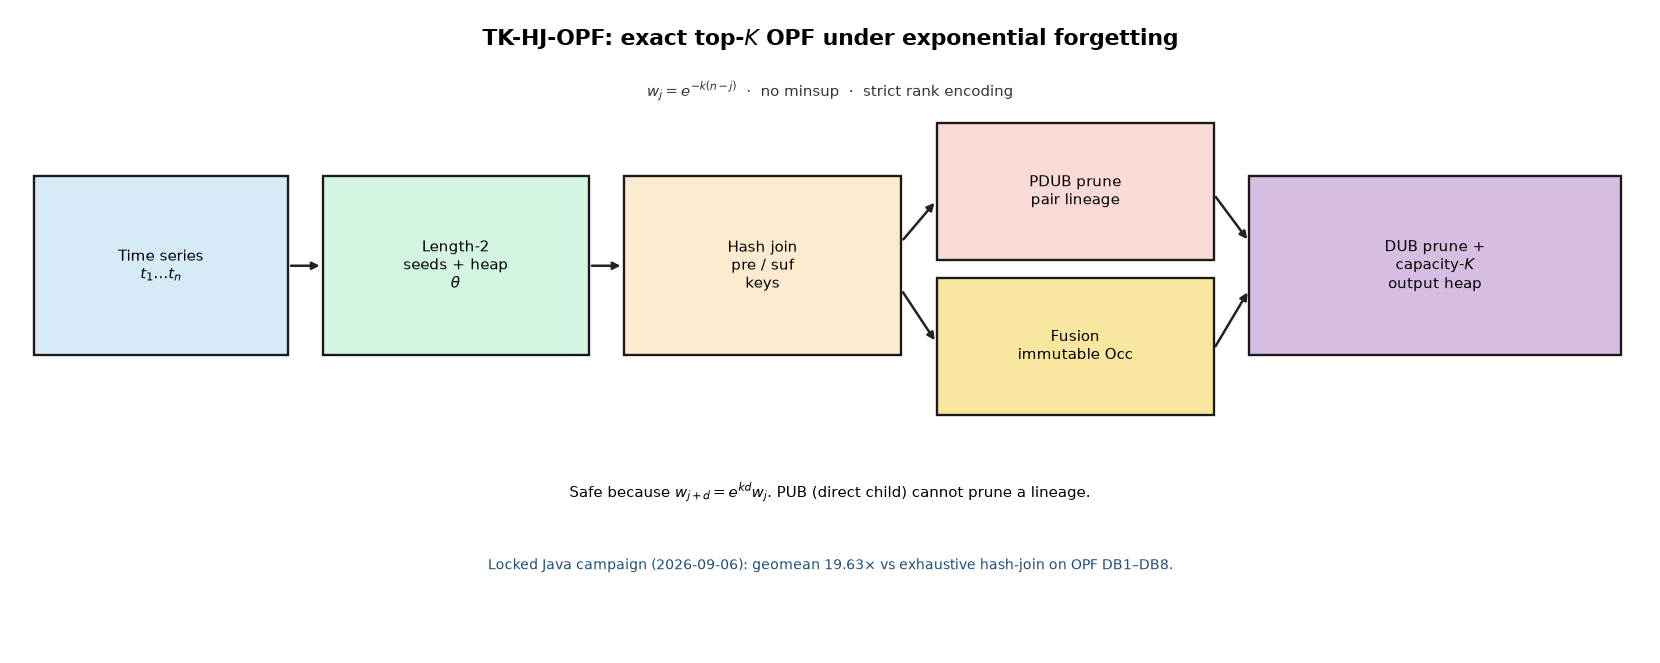
\includegraphics[width=\textwidth]{figures/graphical_abstract.png}
\end{graphicalabstract}

\end{frontmatter}
\hypersetup{pageanchor=true}

\section{Introduction}
\label{sec:intro}

Time-series analysis frequently depends on relative shape rather than absolute amplitude. Order-preserving (OP) matching encodes a window by the ranks of its values~\cite{Kim2014,Crochemore2013}. The idea has grown into a mining family: frequent OP patterns~\cite{Wu2023OPP}, rules~\cite{Wu2023OPR}, approximation~\cite{Li2022AOP}, contrast top-$K$~\cite{Wu2024COPP}, co-occurrence~\cite{Wu2024COP}, outlying occurrences~\cite{Wu2025OUTO}, and stability~\cite{Zhang2026SOPP}. Order-preserving suffix trees (OPST) scale unweighted frequent, maximal, and closed mining~\cite{Li2024Scalable,Li2026Indexing}. Zhou et al.\ review matching and indexing~\cite{Zhou2026Review}.

OPF-Miner addresses temporal relevance~\cite{Li2024OPF}: an occurrence ending at position $j$ in a length-$n$ series receives weight $w_j=e^{-k(n-j)}$. The method remains thresholded; its authors list automatic parameter setting and top-$K$ OPF mining as future work. A naive conversion from minsup search to top-$K$ is unsafe, because forgetting support is not anti-monotone under right extension.

This paper answers that gap \emph{inside the classical fusion architecture}. TK-HJ-OPF (Top-$K$ Hash-Join OPF) uses a hash-indexed prefix--suffix join, immutable occurrence lists, a capacity-$K$ heap, and two forgetting-specific bounds ($\DUB$, $\PDUB$). The contributions are:

\begin{enumerate}
\item The TK-OPF problem: exact global top-$K$ under OPF exponential forgetting, with a deterministic total order and no minsup (Definition~\ref{def:tkopf}).
\item The endpoint-shift identity (Lemma~\ref{lem:shift}) and the bounds $\UB_d$, $\DUB$, $\PUB$, $\PDUB$, including a counterexample that $\PUB$ cannot prune a lineage (Example~\ref{ex:pub}).
\item An output-sensitive hash-indexed fusion algorithm with immutable alignment, together with join soundness, safe pruning under threshold raising, and end-to-end exactness (Theorems~\ref{thm:join}--\ref{thm:exact}).
\item A locked Java campaign on official OPF DB1--DB8: identical canonical top-50 sets across five exact modes, geometric-mean $19.63\times$ over exhaustive hash-join, and a negative ablation ($\PDUB$ safe but not uniformly profitable).
\end{enumerate}

We do not claim the first top-$K$ OP method (COPP-Miner optimizes contrast~\cite{Wu2024COPP}), nor a replacement for unweighted OPST mining~\cite{Li2026Indexing}. TK-HJ-OPF answers: which $K$ OP trends carry the greatest exponentially decayed evidence in one series, under strict (tie-free) windows.

\section{Related work}
\label{sec:related}

OPP-Miner mines frequent OP patterns under minsup~\cite{Wu2023OPP}. Later miners add rules, approximation, co-occurrence, outliers, and stability~\cite{Wu2023OPR,Li2022AOP,Wu2024COP,Wu2025OUTO,Zhang2026SOPP}. COPP-Miner is native top-$K$ but scores class contrast~\cite{Wu2024COPP}. OPF-Miner is the semantic predecessor and remains thresholded~\cite{Li2024OPF}. After an OPST is built, unweighted frequent/maximal/closed OP patterns can be reported in linear time in $n$~\cite{Li2024Scalable,Li2026Indexing}; a static leaf count is not $\sum_j w_j$. Recency weighting outside OP mining includes OIP-Miner~\cite{Wu2025OIP}. Top-$K$ itemset miners such as TFP~\cite{Wang2005TFP} motivate threshold raising; their monotonicities do not transfer. Hash-indexed pair discovery is classical~\cite{Park1995DHP,Balkesen2013}.

\begin{table}[t]
\caption{Closest OP mining lines versus TK-HJ-OPF.}
\label{tab:related}
\centering
\footnotesize
\begin{tabular}{@{}lccc@{}}
\toprule
Work & Forgetting & Native top-$K$ & Distinction \\
\midrule
OPP-Miner~\cite{Wu2023OPP} & no & no & unweighted, minsup \\
OPF-Miner~\cite{Li2024OPF} & yes & no & minsup predecessor \\
COPP-Miner~\cite{Wu2024COPP} & no & yes & contrast score \\
SOPP-Miner~\cite{Zhang2026SOPP} & no & downstream & stability \\
OPST mining~\cite{Li2026Indexing} & no & no & unweighted index \\
\textbf{TK-HJ-OPF} & \textbf{yes} & \textbf{yes} & \textbf{strict fusion} \\
\bottomrule
\end{tabular}
\end{table}

\section{Preliminaries and problem}
\label{sec:prelim}

Notation is $1$-based, matching OPF-Miner~\cite{Li2024OPF}. Companion code uses $0$-based arrays.

\begin{definition}[Time series]
A time series is $\mathbf{t}=(t_1,\ldots,t_n)$ with $t_i\in\mathbb{R}$. Input $\mathrm{NaN}$ and infinities are rejected; $+0$ and $-0$ are identified.
\end{definition}

\begin{definition}[Strict rank encoding]
\label{def:strict}
For a tie-free vector $\mathbf{z}=(z_1,\ldots,z_m)$,
\begin{equation}
\label{eq:strict}
\norm(\mathbf{z})_i=1+\bigl|\{h:z_h<z_i\}\bigr|.
\end{equation}
If $\mathbf{z}$ contains a tie, the window is rejected. A length-$m$ strict OP pattern is a permutation of $\{1,\ldots,m\}$.
\end{definition}

\begin{definition}[Occurrences]
\label{def:occ}
A window of length $m$ ending at $j$ occupies $t_{j-m+1:j}$. For a pattern $\mathbf{p}$,
\begin{equation}
\label{eq:occ}
\Occ(\mathbf{p})=\bigl\{j\in\{m,\ldots,n\}:\norm(t_{j-m+1:j})=\mathbf{p}\bigr\}.
\end{equation}
Forgetting weights depend on the endpoint $j$.
\end{definition}

\begin{definition}[Forgetting weight and support]
\label{def:fsup}
Let $k\ge 0$. The weight of ending position $j$ is
\begin{equation}
\label{eq:wj}
w_j=e^{-k(n-j)},
\end{equation}
so $w_n=1$. The forgetting support is
\begin{equation}
\label{eq:fsup}
\fsup(\mathbf{p})=\sum_{j\in\Occ(\mathbf{p})} w_j.
\end{equation}
If $k=0$, then $\fsup(\mathbf{p})=|\Occ(\mathbf{p})|$.
\end{definition}

\begin{lemma}[Endpoint-shift identity]
\label{lem:shift}
For any valid endpoint $j$ and integer $d\ge 0$ with $j+d\le n$,
\begin{equation}
\label{eq:shift}
w_{j+d}=e^{kd}w_j.
\end{equation}
\end{lemma}
\begin{proof}
$w_{j+d}=e^{-k(n-j-d)}=e^{kd}e^{-k(n-j)}=e^{kd}w_j$.
\end{proof}

\begin{remark}[Non-anti-monotonicity]
\label{rem:nam}
Extending an occurrence of length $m$ starting at $s$ to length $m+1$ multiplies that occurrence's weight by $e^{k}$. The number of occurrences can only drop, but surviving mass becomes heavier, so $\fsup$ need not decrease.
\end{remark}

\begin{definition}[Normalized prefix and suffix]
\label{def:presuf}
For a strict pattern $\mathbf{p}$ of length $m$,
\begin{equation}
\label{eq:presuf}
\pre(\mathbf{p})=\norm(p_1,\ldots,p_{m-1}),\qquad
\suf(\mathbf{p})=\norm(p_2,\ldots,p_m).
\end{equation}
Two length-$m$ patterns are \emph{compatible} when $\suf(\mathbf{p})=\pre(\mathbf{q})$. For a family $F_m$,
\begin{equation}
\label{eq:comp}
\Comp(F_m)=\bigl\{(\mathbf{p},\mathbf{q})\in F_m^2:\suf(\mathbf{p})=\pre(\mathbf{q})\bigr\},
\end{equation}
with $L_m=|F_m|$ and $J_m=|\Comp(F_m)|$.
\end{definition}

\begin{definition}[TK-OPF]
\label{def:tkopf}
Given $\mathbf{t}$, $k\ge 0$, integer $K\ge 1$, and $2\le \ell_{\min}\le \ell_{\max}\le n$, let $\mathcal{P}$ be the set of observed strict patterns with length in $[\ell_{\min},\ell_{\max}]$. Return the first $\min(K,|\mathcal{P}|)$ patterns in the total order: (i)~larger $\fsup$; (ii)~shorter length; (iii)~lexicographically smaller rank sequence. No minsup is supplied.
\end{definition}

A capacity-$K$ min-heap induces a threshold $\theta$: $\theta=0$ while the heap is not full, otherwise $\theta$ is the support of the current worst element. Insertions never decrease $\theta$.

\paragraph{Running example.}
The OPF series
\begin{equation}
\label{eq:running}
\mathbf{t}=(15,32,29,27,34,33,25,20,28,23),\quad n=10,\quad k=0.1,\quad K=5
\end{equation}
is used throughout. For $\mathbf{p}=(1,3,2)$, $\Occ(\mathbf{p})=\{3,6,10\}$ and $\fsup(\mathbf{p})=e^{-0.7}+e^{-0.4}+1=2.166905350$. Table~\ref{tab:top5} is the locked self-test.

\begin{table}[t]
\caption{Exact top-$5$ on the unified running series~\eqref{eq:running}.}
\label{tab:top5}
\centering
\begin{tabular}{@{}rllr@{}}
\toprule
Rank & Pattern & $\Occ(\mathbf{p})$ & $\fsup$ \\
\midrule
1 & $(2,1)$ & $\{3,4,6,7,8,10\}$ & $4.275265960$ \\
2 & $(1,3,2)$ & $\{3,6,10\}$ & $2.166905350$ \\
3 & $(3,2,1)$ & $\{4,7,8\}$ & $2.108360610$ \\
4 & $(1,2)$ & $\{2,5,9\}$ & $1.960697042$ \\
5 & $(2,1,3)$ & $\{5,9\}$ & $1.511368078$ \\
\bottomrule
\end{tabular}
\end{table}

\section{Output-sensitive indexed fusion}
\label{sec:join}

\begin{lemma}[Direct rank projection]
\label{lem:proj}
Let $\mathbf{p}$ be a permutation of $\{1,\ldots,m\}$. Removing rank $x$ sends every remaining rank $v>x$ to $v-1$ and leaves $v<x$ unchanged. Thus $\pre(\mathbf{p})$ and $\suf(\mathbf{p})$ each take $O(m)$ time.
\end{lemma}
\begin{proof}
Removing $x$ removes exactly one smaller predecessor of every $v>x$. Removing $p_m$ (resp.\ $p_1$) yields the prefix (resp.\ suffix).
\end{proof}

\begin{lemma}[Faithful compatibility key]
\label{lem:key}
Under Definition~\ref{def:strict}, $\suf(\mathbf{p})=\pre(\mathbf{q})$ iff the $m-1$ overlapping positions are order-isomorphic.
\end{lemma}
\begin{proof}
A strict rank vector canonically encodes a strict total order.
\end{proof}

\begin{theorem}[Join soundness and completeness]
\label{thm:join}
Inserting every $\mathbf{q}\in F_m$ into a multimap keyed by $\pre(\mathbf{q})$ and probing with $\suf(\mathbf{p})$ emits exactly $\Comp(F_m)$.
\end{theorem}
\begin{proof}
Emitted pairs have equal keys, hence are compatible. Conversely, a compatible $\mathbf{q}$ lies in exactly the bucket probed by $\mathbf{p}$.
\end{proof}

Expected hash work is $O(L_m+J_m)$ after keys exist; Lemma~\ref{lem:proj} costs $O(mL_m)$ if keys are not cached.

\begin{algorithm}[t]
\caption{HJ-Compatible: emit $\Comp(F_m)$}
\label{alg:hj}
\begin{algorithmic}[1]
\Require family $F_m$ of length-$m$ strict patterns with cached $\pre/\suf$ keys
\State $H\leftarrow$ empty multimap
\For{each $\mathbf{q}\in F_m$}
  \State append $\mathbf{q}$ to $H[\pre(\mathbf{q})]$
\EndFor
\For{each $\mathbf{p}\in F_m$}
  \For{each $\mathbf{q}$ in $H.\mathrm{lookup}(\suf(\mathbf{p}))$}
    \State emit $(\mathbf{p},\mathbf{q})$
  \EndFor
\EndFor
\end{algorithmic}
\end{algorithm}

\section{Forgetting-specific upper bounds}
\label{sec:bounds}

A \emph{right-descendant at depth $d$} of a length-$m$ pattern $\mathbf{p}$ is a length-$(m+d)$ pattern whose first $m$ positions are order-isomorphic to $\mathbf{p}$.

\begin{theorem}[Depth-$d$ descendant bound]
\label{thm:ubd}
For any right-descendant $\mathbf{x}$ of $\mathbf{p}$ at depth $d$,
\begin{equation}
\label{eq:ubd}
\fsup(\mathbf{x})\le \UB_d(\mathbf{p})
:=e^{kd}\sum_{\substack{o\in\Occ(\mathbf{p})\\ o\le n-d}} w_o.
\end{equation}
\end{theorem}
\begin{proof}
Every occurrence of $\mathbf{x}$ ending at $j$ induces a unique prefix occurrence of $\mathbf{p}$ ending at $o=j-d$ with $o\le n-d$. If $S$ is the subset realizing $\mathbf{x}$, Lemma~\ref{lem:shift} gives $\fsup(\mathbf{x})=e^{kd}\sum_{o\in S}w_o$, which is at most~\eqref{eq:ubd}.
\end{proof}

\begin{definition}[Descendant Upper Bound]
\label{def:dub}
For $D=\ell_{\max}-|\mathbf{p}|$,
\begin{equation}
\label{eq:dub}
\DUB(\mathbf{p})=\max_{0\le d\le D}\UB_d(\mathbf{p}).
\end{equation}
\end{definition}

\begin{corollary}[Safe subtree pruning]
\label{cor:dub}
If the heap is full and $\DUB(\mathbf{p})<\theta$, no allowed right-descendant of $\mathbf{p}$ can belong to the final top-$K$. The inequality is strict so that support ties remain available for the secondary order.
\end{corollary}

\begin{proposition}[Efficient DUB evaluation]
\label{prop:dub}
Let $o_1<\cdots<o_s$ be sorted endpoints and $W_i=\sum_{h\le i}w_{o_h}$. The active set in $\UB_d$ changes only when $d$ crosses $n-o_i$. Between changes the weighted sum is constant while $e^{kd}$ increases, so maxima occur at interval right endpoints. It suffices to evaluate $d=0$, $d=D$, and breakpoints $d=n-o_i$.
\end{proposition}

\begin{theorem}[Immediate-child PUB]
\label{thm:pub}
Let $\mathbf{p},\mathbf{q}$ be compatible length-$m$ patterns and $\mathbf{r}$ any direct length-$(m+1)$ child. Then
\begin{equation}
\label{eq:pub}
\fsup(\mathbf{r})\le \PUB(\mathbf{p},\mathbf{q})
:=\min\bigl\{e^{k}\fsup(\mathbf{p}),\,\fsup(\mathbf{q})\bigr\}.
\end{equation}
\end{theorem}
\begin{proof}
A child occurrence ending at $j$ maps injectively to a prefix occurrence of $\mathbf{p}$ at $j-1$ and a suffix occurrence of $\mathbf{q}$ at $j$. Lemma~\ref{lem:shift} gives $\fsup(\mathbf{r})\le e^{k}\fsup(\mathbf{p})$ and $\fsup(\mathbf{r})\le\fsup(\mathbf{q})$.
\end{proof}

PUB is safe for the direct child only.

\begin{example}[Naive PUB lineage pruning is incorrect]
\label{ex:pub}
On~\eqref{eq:running} let $\mathbf{p}=(1,4,3,2)$, $\Occ(\mathbf{p})=\{4\}$, $\mathbf{q}=(3,2,1,4)$, $\Occ(\mathbf{q})=\{5\}$. Then $\fsup(\mathbf{p})=e^{-0.6}=0.548812$, $\fsup(\mathbf{q})=e^{-0.5}=0.606531$, the direct child $\mathbf{r}=(1,4,3,2,5)$ has support $0.606531$, and $\PUB=0.606531$. The later descendant $\mathbf{x}=(1,8,7,5,10,9,4,2,6,3)$ occurs at endpoint $10$ with support $1.0$. A temporary threshold $0.8$ would drop the pair under $\PUB$ and lose $\mathbf{x}$.
\end{example}

\begin{theorem}[Depth-$d$ pair-descendant bound]
\label{thm:pdb}
Let $\mathbf{x}$ be obtained from a compatible pair $(\mathbf{p},\mathbf{q})$ by one direct child and $d\ge 0$ right extensions. Then
\begin{equation}
\label{eq:pdb}
\fsup(\mathbf{x})\le \min\bigl\{\UB_{d+1}(\mathbf{p}),\,\UB_d(\mathbf{q})\bigr\}.
\end{equation}
\end{theorem}
\begin{proof}
An occurrence of $\mathbf{x}$ ending at $j$ realizes $\mathbf{p}$ at $j-(d+1)$ and $\mathbf{q}$ at $j-d$. Both maps are injective; apply Theorem~\ref{thm:ubd}.
\end{proof}

\begin{definition}[Pair-Descendant Upper Bound]
\label{def:pdub}
With $D=\ell_{\max}-(m+1)$,
\begin{equation}
\label{eq:pdub}
\PDUB_D(\mathbf{p},\mathbf{q})
=\max_{0\le d\le D}\min\bigl\{\UB_{d+1}(\mathbf{p}),\,\UB_d(\mathbf{q})\bigr\}.
\end{equation}
\end{definition}

\begin{corollary}[Safe pre-fusion pruning]
\label{cor:pdub}
If the heap is full and $\PDUB_D(\mathbf{p},\mathbf{q})<\theta$, the pair can be discarded before occurrence alignment.
\end{corollary}

On Example~\ref{ex:pub}, $\PDUB_5=1.0$, so the pair survives any threshold up to $1.0$. Once $\mathbf{p}=(1,4,3,2)$ is materialized, $\DUB(\mathbf{p})=1.0$ is compared with the live heap threshold.

\section{The TK-HJ-OPF algorithm}
\label{sec:alg}

\begin{lemma}[Exact immutable fusion]
\label{lem:fusion}
For a compatible pair, immutable occurrence alignment enumerates exactly the strict OP occurrences of each generated child, and summing $w_j$ equals Definition~\ref{def:fsup}.
\end{lemma}
\begin{proof}
A child occurrence ending at $j$ has a unique prefix endpoint $j-1$ and suffix endpoint $j$. Conversely, an aligned compatible pair fixes the overlap order; comparing the first and last values completes the strict total order, or the window is rejected on a tie.
\end{proof}

\begin{algorithm}[t]
\caption{TK-HJ-OPF}
\label{alg:tkhj}
\begin{algorithmic}[1]
\Require series $\mathbf{t}$, decimal $k\ge 0$, integer $K$, $[\ell_{\min},\ell_{\max}]$
\State $F\leftarrow$ all length-$\ell_{\min}$ strict patterns with exact $\fsup$
\State $H\leftarrow$ capacity-$K$ heap on $F$; $\theta\leftarrow$ heap threshold
\State $\mathit{Front}\leftarrow\{p\in F: H\text{ not full or }\DUB(p)\ge\theta\}$
\For{$m=\ell_{\min},\ldots,\ell_{\max}-1$}
  \State $J\leftarrow$ hash-join $\Comp(\mathit{Front})$ \Comment{Theorem~\ref{thm:join}}
  \State $\mathit{Next}\leftarrow\emptyset$
  \For{each pair $(\mathbf{p},\mathbf{q})\in J$}
    \If{$H$ full and $\PDUB(\mathbf{p},\mathbf{q})<\theta$}
      \State \textbf{continue}
    \EndIf
    \For{each child $\mathbf{r}$ of exact fusion of $(\mathbf{p},\mathbf{q})$}
      \State score $\mathbf{r}$; possibly insert $H$ and raise $\theta$
      \If{$|\mathbf{r}|<\ell_{\max}$ and ($H$ not full or $\DUB(\mathbf{r})\ge\theta$)}
        \State add $\mathbf{r}$ to $\mathit{Next}$
      \EndIf
    \EndFor
  \EndFor
  \State $\mathit{Front}\leftarrow\mathit{Next}$
\EndFor
\State \Return $H$
\end{algorithmic}
\end{algorithm}

\paragraph{Worked trace.}
On~\eqref{eq:running}, length $2$ inserts $(2,1)$ (support $4.275266$) and $(1,2)$ ($1.960697$). For $\mathbf{p}=(1,3,2)$, $\suf(\mathbf{p})=(2,1)=\pre(3,2,1)$, so the join emits that pair. Fusion produces $(1,4,3,2)$ at endpoint $4$ ($0.548812$) and $(2,4,3,1)$ at $7$ ($0.740818$). Once five patterns exist, $\theta=1.511368$. The heap returns Table~\ref{tab:top5}.

\section{Correctness and complexity}
\label{sec:correct}

\begin{lemma}[Threshold monotonicity]
\label{lem:theta}
If $\theta_t$ is the heap threshold at a prune time and $\theta_f$ the threshold at termination, then $\theta_f\ge\theta_t$.
\end{lemma}
\begin{proof}
The heap replaces its worst element only with a strictly better pattern under Definition~\ref{def:tkopf}, so the worst-in-heap support never decreases after the heap is full.
\end{proof}

\begin{theorem}[Safe pruning]
\label{thm:prune}
Any pair lineage pruned by $\PDUB$ and any subtree pruned by $\DUB$ contains no final top-$K$ pattern.
\end{theorem}
\begin{proof}
Corollaries~\ref{cor:pdub} and~\ref{cor:dub} bound discarded patterns strictly below $\theta_t$. Lemma~\ref{lem:theta} gives $\theta_f\ge\theta_t$.
\end{proof}

\begin{theorem}[Soundness and completeness]
\label{thm:exact}
Under strict OP semantics and exact real-valued support, Algorithm~\ref{alg:tkhj} returns exactly the deterministic top-$K$ patterns in $[\ell_{\min},\ell_{\max}]$.
\end{theorem}
\begin{proof}
\emph{Soundness.} Lemma~\ref{lem:fusion}: every heap insertion uses an exact occurrence list.

\emph{Completeness.} Let $\mathbf{x}$ be a final top-$K$ pattern of length $m+1>2$, $\mathbf{p}=\norm(x_1,\ldots,x_m)$, $\mathbf{q}=\norm(x_2,\ldots,x_{m+1})$. Theorem~\ref{thm:ubd} gives $\fsup(\mathbf{x})\le\DUB(\mathbf{p})$ and $\fsup(\mathbf{x})\le\DUB(\mathbf{q})$. Then $\theta_t\le\theta_f\le\fsup(\mathbf{x})$, so neither parent is $\DUB$-pruned. Theorem~\ref{thm:join} emits the pair; $\PDUB\ge\fsup(\mathbf{x})\ge\theta_t$, so the pair is not pruned. Lemma~\ref{lem:fusion} generates $\mathbf{x}$. Induction from length-$\ell_{\min}$ seeds, plus a capacity-$K$ heap, yields the global top $K$.
\end{proof}

Let $P_m$ be patterns surviving to generation $m$, $B_m\subseteq J_m$ pairs rejected by $\PDUB$, $A(\mathbf{p},\mathbf{q})$ alignment comparisons, $S$ scored patterns, and $C_{\mathrm{PD}}$, $C_{\mathrm{DUB}}$ bound-evaluation costs.

\begin{theorem}[Expected work]
\label{thm:work}
Ignoring JVM constants, expected work decomposes as
\begin{equation}
\label{eq:work}
\begin{aligned}
&O\Bigl(\textstyle\sum_m(mL_m+L_m+J_m)+C_{\mathrm{PD}}\\
&\qquad+\textstyle\sum_m\sum_{(\mathbf{p},\mathbf{q})\in J_m\setminus B_m}A(\mathbf{p},\mathbf{q})
+C_{\mathrm{DUB}}+S\log K\Bigr).
\end{aligned}
\end{equation}
\end{theorem}

Equation~\eqref{eq:work} is search-space sensitive, not a polynomial in $n$ alone. No claim of asymptotic global optimality is made.

\section{Experimental verification}
\label{sec:exp}

All numbers were measured on 6~September 2026 on one host. We do not reuse ARM64 wall-clock tables from an earlier laptop campaign.

\begin{table}[t]
\caption{Locked environment.}
\label{tab:env}
\centering
\begin{tabular}{@{}ll@{}}
\toprule
Item & Value \\
\midrule
CPU & Intel Core i5-8250U, 4c/8t, $1.60$\,GHz \\
Memory & $32$\,GB \\
OS & Windows 11, build 26200, amd64 \\
Java & Temurin OpenJDK $25.0.3$; \texttt{javac --release 21} \\
JVM & \texttt{-Xms2g -Xmx8g}; one JVM \\
Timing & \texttt{System.nanoTime()} around \texttt{mine()} \\
Central grid & 5 warmups + 10 measured runs \\
\bottomrule
\end{tabular}
\end{table}

Five exact modes: \texttt{hjtopk} (exhaustive join, no search pruning), \texttt{tk-no-bounds}, \texttt{tk-no-dub} ($\PDUB$ only), \texttt{tk-no-pdub} ($\DUB$ only), \texttt{tk} (both). Official series SHA-256 match the OPF-Miner suite~\cite{OPFCode2024} (Table~\ref{tab:data}). Geometric means follow Fleming and Wallace~\cite{Fleming1986}.

\begin{table}[t]
\caption{Official OPF-Miner series~\cite{OPFCode2024}.}
\label{tab:data}
\centering
\footnotesize
\begin{tabular}{@{}llr@{}}
\toprule
ID & Dataset & $n$ \\
\midrule
DB1 & Amazon & $5842$ \\
DB2 & Russell 2000 & $8141$ \\
DB3 & Nasdaq & $12279$ \\
DB4 & S\&P 500 & $23046$ \\
DB5 & NYSE & $60000$ \\
DB6 & CL.US & $10305$ \\
DB7 & HPQ.US & $12075$ \\
DB8 & GE.US & $14058$ \\
\bottomrule
\end{tabular}
\end{table}

\subsection{Exactness}
Java \texttt{tk}/\texttt{hjtopk} and the single-file companion return Table~\ref{tab:top5} (tolerance $10^{-10}$). \texttt{RandomizedSelf\-Test} (seed~20260818) completed $2400$ exact comparisons against window enumeration. Canonical SHA-256 of the top-50 set is identical across all five modes on all eight official files.

\subsection{Central DB1--DB8}
Table~\ref{tab:central} reports $K=50$, $\ell_{\max}=12$, $k=1/n$. Full TK-HJ-OPF is $6.88$--$35.66\times$ faster than exhaustive HJ (geomean $19.63$). $\DUB$-only is fastest on seven of eight datasets; full TK-HJ is slightly faster on NYSE. $\PDUB$ is safe but not uniformly cheaper than $\DUB$-only.

\begin{table}[t]
\caption{Central campaign, $K=50$, $\ell_{\max}=12$, $k=1/n$. Median ms, ten measured runs after five warmups.}
\label{tab:central}
\centering
\small
\setlength{\tabcolsep}{4pt}
\resizebox{\textwidth}{!}{%
\begin{tabular}{@{}lrrrrrr@{}}
\toprule
Dataset & $n$ & HJ & DUB-only & Full TK & HJ/TK & HJ/DUB \\
\midrule
Amazon & 5842 & 69.941 & \textbf{1.859} & 1.961 & 35.66$\times$ & 37.62$\times$ \\
Russell 2000 & 8141 & 64.229 & \textbf{2.542} & 2.669 & 24.07$\times$ & 25.27$\times$ \\
Nasdaq & 12279 & 89.371 & \textbf{3.349} & 3.508 & 25.48$\times$ & 26.68$\times$ \\
S\&P 500 & 23046 & 146.488 & \textbf{5.622} & 6.135 & 23.88$\times$ & 26.05$\times$ \\
NYSE & 60000 & 96.432 & 14.676 & \textbf{14.026} & 6.88$\times$ & 6.57$\times$ \\
CL.US & 10305 & 49.993 & \textbf{2.318} & 2.399 & 20.84$\times$ & 21.56$\times$ \\
HPQ.US & 12075 & 53.981 & \textbf{2.801} & 2.895 & 18.64$\times$ & 19.27$\times$ \\
GE.US & 14058 & 50.950 & \textbf{3.199} & 3.219 & 15.83$\times$ & 15.93$\times$ \\
\midrule
Geomean & & & & & 19.63$\times$ & 20.29$\times$ \\
\bottomrule
\end{tabular}%
}
\end{table}

On Amazon the IQR of full TK is $[1.878,2.521]$\,ms versus $[63.541,83.517]$\,ms for HJ. Figures~\ref{fig:runtime} and~\ref{fig:speedup} show the five-mode runtime (log scale) and per-dataset HJ/TK speedup.

\begin{figure}[t]
\centering
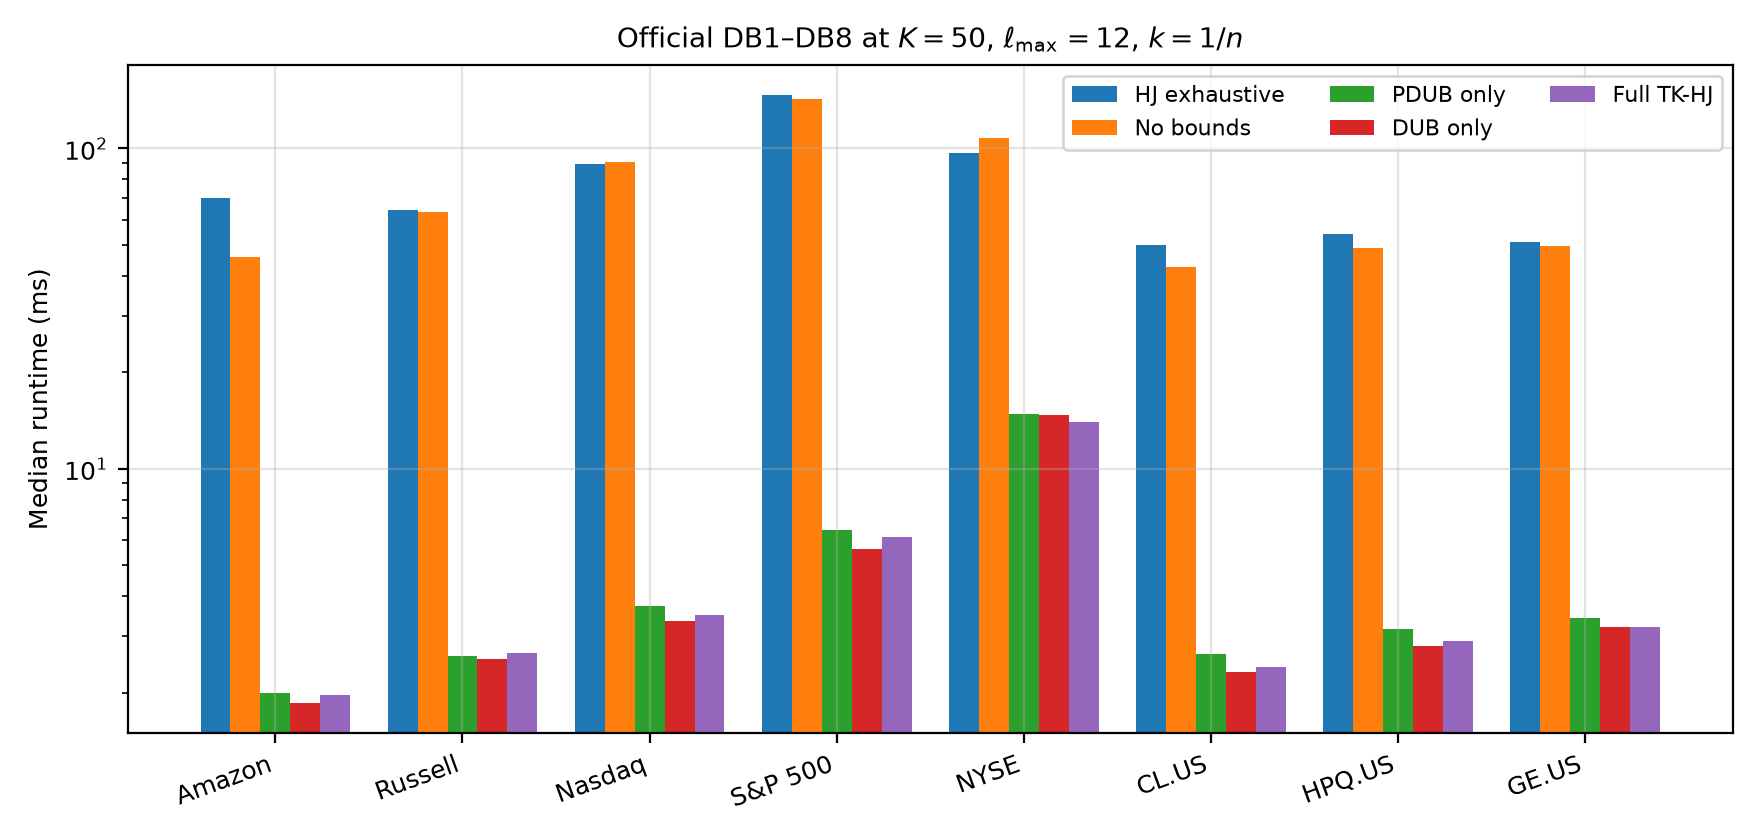
\includegraphics[width=\linewidth]{figures/official_runtime.png}
\caption{Median runtime of five exact variants on official DB1--DB8 at $K=50$, $\ell_{\max}=12$, $k=1/n$. Logarithmic $y$-axis.}
\label{fig:runtime}
\end{figure}

\begin{figure}[t]
\centering
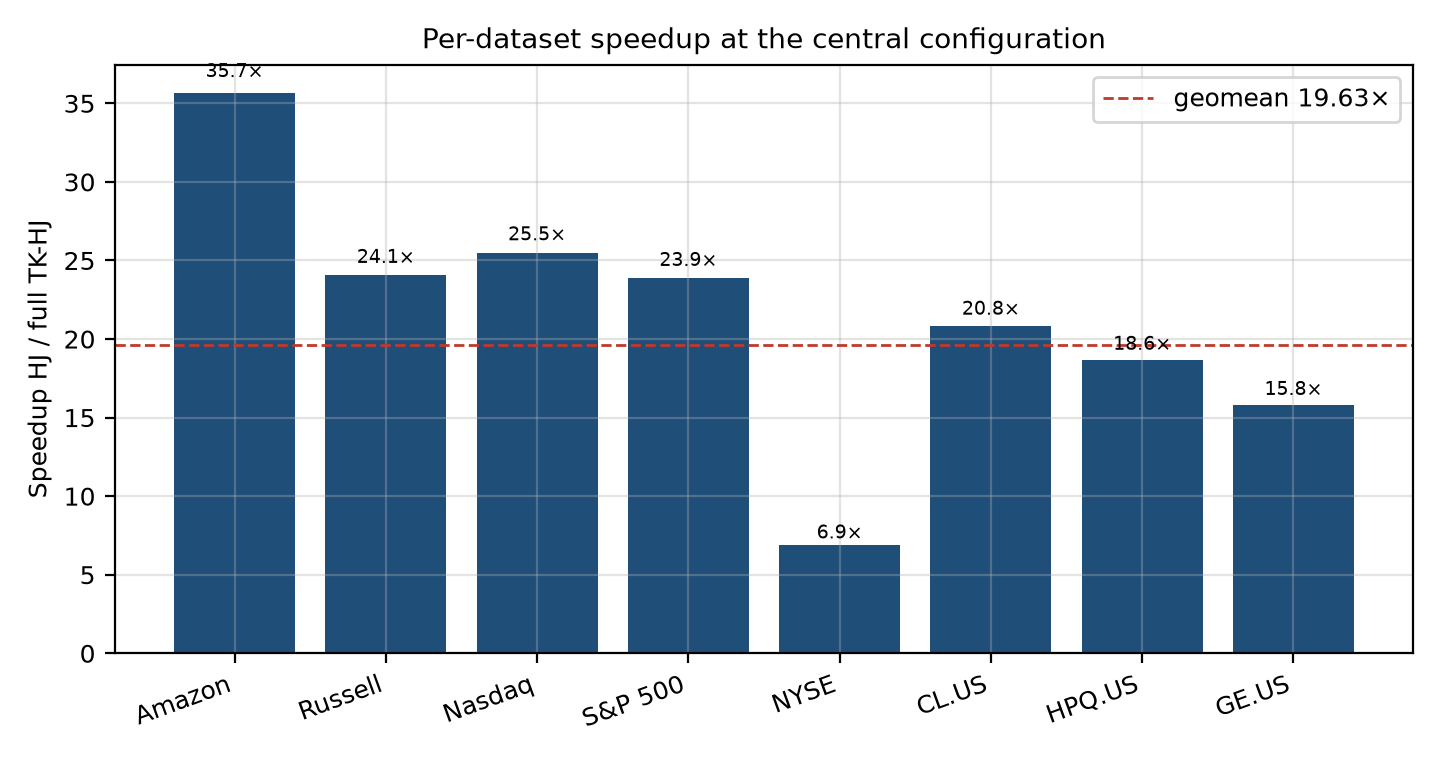
\includegraphics[width=\linewidth]{figures/official_speedup.png}
\caption{Per-dataset speedup of full TK-HJ-OPF over exhaustive HJ at the central configuration. Dashed line: geometric mean $19.63\times$.}
\label{fig:speedup}
\end{figure}

The principal gain is pruning, not hashing alone. Table~\ref{tab:pairs} records median pair-discovery and alignment counters at the same central cell. Exhaustive HJ on Amazon emits $20878$ pair attempts and $39128$ compatible pairs, versus $84$ and $232$ under full TK-HJ-OPF; aligned occurrence comparisons fall from $261668$ to $95480$. $\PDUB$ prunes $79$ pairs and $\DUB$ prunes $105$ child branches on that series. No-bound variants remain close to exhaustive HJ in wall-clock (Table~\ref{tab:central} and \texttt{timing.csv}), so the speedup is explained by raising $\theta$ and discarding hopeless regions.

\begin{table}[t]
\caption{Median search-space counters at $K=50$, $\ell_{\max}=12$, $k=1/n$. Pair attempts and compatible pairs are hash-join events; aligned checks are occurrence-list comparisons.}
\label{tab:pairs}
\centering
\footnotesize
\setlength{\tabcolsep}{3.5pt}
\resizebox{\textwidth}{!}{%
\begin{tabular}{@{}lrrrrrr@{}}
\toprule
Dataset & HJ pairs & HJ aligned & TK pairs & TK aligned & PDUB prunes & DUB prunes \\
\midrule
Amazon & 20878 & 261668 & 84 & 95480 & 79 & 105 \\
Russell 2000 & 27203 & 415273 & 84 & 138862 & 70 & 106 \\
Nasdaq & 35427 & 663551 & 82 & 206420 & 74 & 99 \\
S\&P 500 & 54459 & 1181569 & 81 & 374157 & 71 & 108 \\
NYSE & 27873 & 2778106 & 81 & 934774 & 95 & 104 \\
CL.US & 19036 & 316928 & 78 & 135185 & 68 & 105 \\
HPQ.US & 20077 & 377322 & 77 & 162972 & 61 & 112 \\
GE.US & 16697 & 330778 & 83 & 156966 & 77 & 107 \\
\bottomrule
\end{tabular}%
}
\end{table}

\subsection{Sensitivity}
Sweeps ran in the same JVM after the central grid; they support trends, not a second locked table. On Amazon at $\ell_{\max}=12$, HJ/TK falls from $61.3\times$ at $K=10$ to $8.0\times$ at $K=500$ (Fig.~\ref{fig:ksens}). Exhaustive HJ on Amazon grows with $\ell_{\max}$ ($10.7$\,ms at $8$, $37.7$ at $12$, $92.0$ at $16$) while full TK stays near $2$\,ms. Varying $k\in\{0.25,0.5,1,2,4\}/n$ at $K=50$ did not change the runtime regime on Amazon or GE.US.

\begin{figure}[t]
\centering
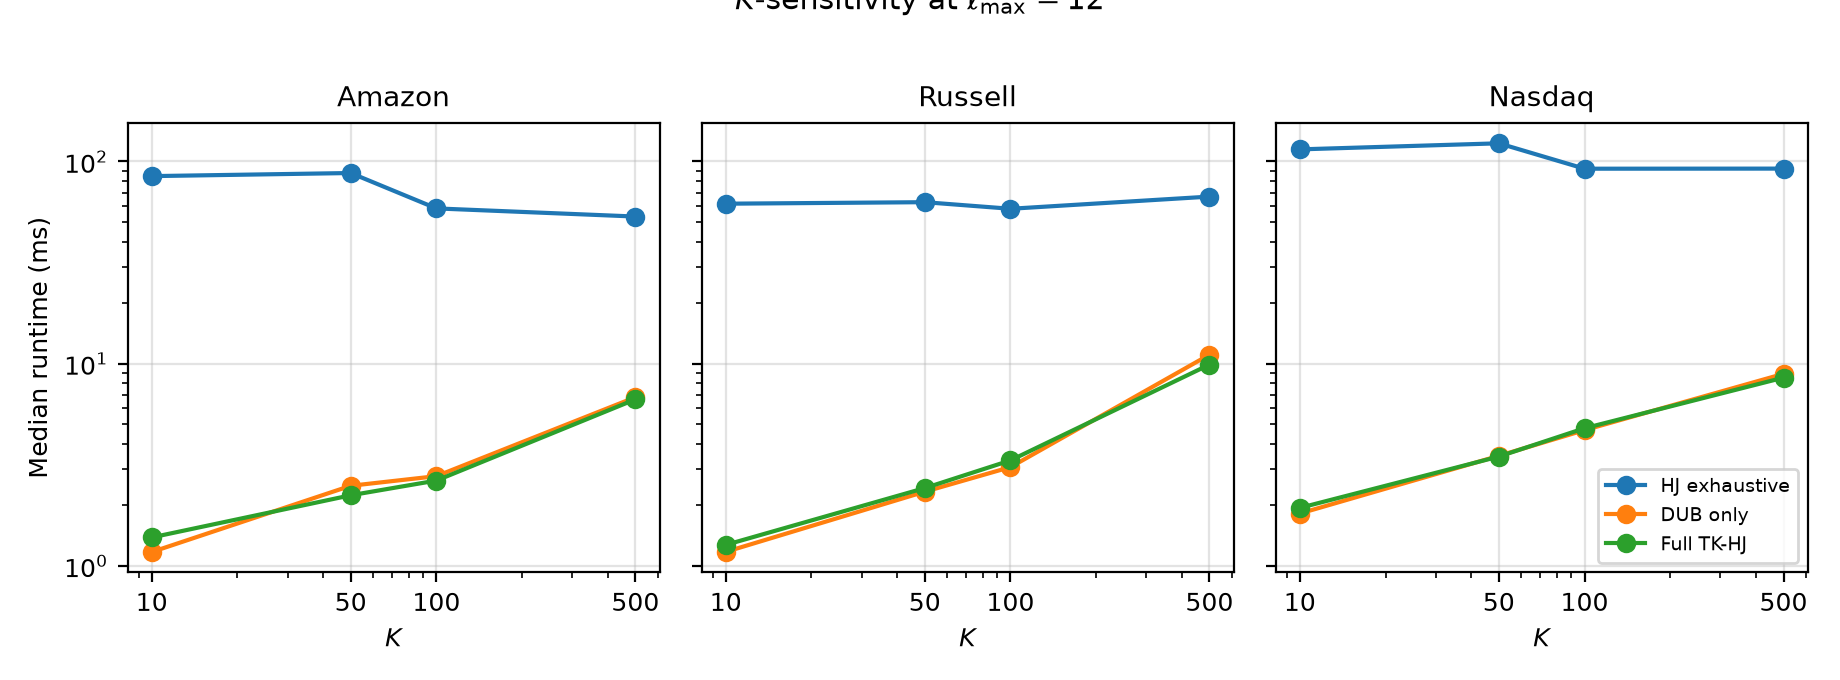
\includegraphics[width=\linewidth]{figures/official_K_sensitivity.png}
\caption{$K$-sensitivity on Amazon, Russell 2000, and Nasdaq at $\ell_{\max}=12$ (log--log). Exhaustive HJ is comparatively insensitive to $K$; full TK-HJ-OPF and DUB-only become slower as the heap threshold rises more slowly.}
\label{fig:ksens}
\end{figure}

\subsection{Public tie-rich series (SILSO)}
\label{sec:silso}
To step outside the financial OPF suite we ran the same host, JVM flags, and protocol (5 warmups + 10 measured, $K=50$, $\ell_{\max}=12$, $k=1/n$) on WDC-SILSO daily total sunspot number v2.0~\cite{SILSO2026}. Missing markers (SSN ${<}0$) were dropped, leaving $n=72967$ integer counts. Strict encoding rejects tied windows, so this series stresses the tie-rejection path.

Median milliseconds: exhaustive HJ $191.797$, DUB-only $12.325$, full TK-HJ $12.768$ (HJ/TK $=15.02\times$). DUB-only is again slightly faster than full TK-HJ. A Windows Working-Set sample of the \emph{whole} public-campaign JVM (all three modes in one process, \texttt{-Xms2g -Xmx8g}) peaked at $1303.5$\,MB. That number is process-level, not a per-algorithm OS Peak RSS, and is not compared with Table~\ref{tab:central}.

\subsection{Memory reporting}
Campaign CSVs record diagnostic in-process JVM heap
(\texttt{totalMemory}${}-{}$\texttt{freeMemory}) in column \texttt{peak\_heap\_mb}.
Those values are \emph{not} OS Peak RSS and were collected in one long-lived JVM, so they must not be read as a cross-algorithm memory ranking. A per-mode RSS campaign in a fresh process remains future work.

\subsection{What is not claimed}
No per-algorithm OS Peak RSS. No FRED timings on this host. No OPST runtime. No architecture-independent speedup.

\section{Discussion}
\label{sec:disc}

TK-HJ-OPF is a weighted ranking method, not a general replacement for OP mining. Unweighted maximal or closed discovery at very large scale is the natural home of OPST indexing~\cite{Li2026Indexing}. Class discrimination is the home of COPP-Miner~\cite{Wu2024COPP}. Stability of occurrence distributions is the home of SOPP-Miner~\cite{Zhang2026SOPP}. TK-HJ-OPF answers: which $K$ OP trends carry the greatest exponentially decayed evidence in one series, under strict windows.

The theoretical core is that a surviving occurrence becomes heavier under right extension (Lemma~\ref{lem:shift}). $\DUB$ repairs subtree pruning; $\PUB$ is valid only for a direct child (Example~\ref{ex:pub}); $\PDUB$ repairs pair-lineage pruning. The experiments add a second lesson: a safe earlier bound is not necessarily faster. Unconditional $\PDUB$ reduces alignment counts (Table~\ref{tab:pairs}) and can still lose to $\DUB$-only in wall-clock (Table~\ref{tab:central}). A practical next step is an adaptive rule that compares expected alignment cost with expected $\PDUB$ cost from list sizes, depth, and current $\theta$.

\section{Threats to validity}
\label{sec:threats}

Novelty is limited to exact global top-$K$ under OPF forgetting with the proposed fusion bounds; we do not claim the first scalable OP method. A keyword search (IEEE Xplore / arXiv / TKDE, 6--7~September 2026; queries in \texttt{NOVELTY\_SEARCH.md}) found OPF-Miner (minsup), COPP-Miner (contrast top-$K$), OPST unweighted mining, and OIP-Miner (non-OP forgetting), but no published exact global top-$K$ OPF fusion miner. That log is not a non-existence proof.

Mathematics assumes exact reals; Java uses IEEE-754 $\texttt{Math.exp}$ with a conservative ULP prune guard. One x86 laptop and $\ell_{\max}\le 16$ do not establish architecture-independent or unrestricted-length scalability. Official files are financial; SILSO is tie-rich integers under strict rejection.

\section{Conclusion}
\label{sec:conclusion}

TK-HJ-OPF solves exact threshold-free top-$K$ OPF inside fusion: hash-indexed compatible pairs, immutable alignment, and $\DUB$/$\PDUB$ derived from $w_{j+d}=e^{kd}w_j$. Example~\ref{ex:pub} shows that $\PUB$ cannot prune a lineage. On this host, at $K=50$ and $\ell_{\max}=12$, full TK-HJ-OPF is a $19.63\times$ geometric-mean improvement over exhaustive hash-join on DB1--DB8, with identical canonical top-50 sets, and $15.02\times$ on SILSO ($n=72967$). $\DUB$ is the consistent accelerator and unconditional $\PDUB$ is not uniformly profitable. Future work includes adaptive $\PDUB$ activation, streaming TK-OPF, weighted OPST indexing, and a dedicated per-mode OS RSS campaign.

\section*{Data and code}
Java~21 sources, the campaign runner, \texttt{timing.csv}, and \texttt{canonical.tsv} are in the companion repository \url{https://github.com/Porcupine1805/TK-HJ-OPF}. Official OPF-Miner series are not redistributed; SHA-256 checksums are in \texttt{DATASETS.md}.

\section*{CRediT authorship contribution statement}
Khac-Chien Nguyen: conceptualization, methodology, software, validation, writing --- original draft, writing --- review and editing (corresponding author).
Nhut-Minh Bui: methodology, software, validation, writing --- review and editing.
Cong-Phat Tran: methodology, software, validation, data curation, writing --- review and editing.
Roles can be revised by the authors before journal submission.

\section*{Declaration of competing interest}
The authors declare that they have no known competing financial interests or personal relationships that could have appeared to influence the work reported in this paper.

\bibliographystyle{elsarticle-num}
\bibliography{references}
\end{document}
